Soit la fonction $f$ définie sur l'intervalle $]1; +\infty[$ par \[f(x) = x - \ln (x - 1).\]
%
On considère la suite $\left(u_n\right)$ de terme initial $u_0 = 10$ et telle que $u_{n+1} = f\left(u_n\right)$ pour tout entier naturel $n$.

\bigskip

\textbf{Partie I :}

\medskip

La feuille de calcul ci-dessous a permis d'obtenir des valeurs approchées des premiers termes de la suite $\left(u_n\right)$.

\begin{center}
	%TABLEUR
	\begin{tikzpicture}
		\tableur*[10]{A/4cm,B/4cm}
		\celtxt*[c]{A}{1}{$n$}
		\celtxt*[c]{B}{1}{$u_n$}
		\foreach \A in {2,3,...,10}{%
			\FPeval{nba}{clip(\A-2)}
			\celtxt*[c]{A}{\A}{$\nba$}
		}
		\foreach \L/\V in {2/10,3/\num{7,80277542},4/\num{5,88544474},5/\num{4,29918442},6/\num{3,10550913},7/\num{2,36095182},8/\num{2,0527675},9/\num{2,00134509},10/\num{2,0000009}}{%
			\celtxt*[c]{B}{\L}{\V}
		}
	\end{tikzpicture}
\end{center}

\begin{enumerate}
	\item Quelle formule a été saisie dans la cellule B3 pour permettre de $\left(u_n\right)$ par recopie vers le bas ?
	\item À l'aide de ces valeurs, conjecturer le sens de variation et la le calcul des valeurs approchées limite de la suite $\left(u_n\right)$.
\end{enumerate}

\textbf{Partie II :}

\medskip

On rappelle que la fonction $f$ est définie sur l'intervalle $]1; +\infty[$ par \[f(x) = x - \ln (x - 1).\]

\begin{enumerate}
	\item Calculer $\displaystyle\lim_{x \to 1} f(x)$. On admettra que $\displaystyle\lim_{x \to + \infty} f(x) = + \infty$.
	\item  
	\begin{enumerate}
		\item Soit $f'$ la fonction dérivée de $f$. Montrer que pour tout $x \in ]1; +\infty[$, $f'(x) = \dfrac{x - 2}{x - 1}$.
		\item En déduire le tableau des variations de $f$ sur l'intervalle $]1; +\infty[$, complété par les limites.
		\item Justifier que pour tout $x \geqslant  2$, $f(x) \geqslant  2$.
	\end{enumerate}
\end{enumerate}

\textbf{Partie III :}

\begin{enumerate}
	\item En utilisant les résultats de la partie \textbf{II}, démontrer par récurrence que $u_n \geqslant  2$ pour tout entier naturel $n$.
	\item Montrer que la suite $\left(u_n\right)$ est décroissante.
	\item En déduire que la suite $\left(u_n\right)$ est convergente. On note $\ell$ sa limite.
	\item On admet que $\ell$ vérifie $f(\ell) = \ell$. Donner la valeur de $\ell$.
\end{enumerate}